% This template was designed by Ruben De Smet. Visit his website at https://gitlab.com/rubdos/texlive-vub

\documentclass{beamer}

\usepackage{textpos}
\usepackage{selinput}
\usepackage{fontspec}
\usepackage{tikz}
\usepackage{graphicx}
\usepackage{minted}
\usepackage{svg}

\usefonttheme{professionalfonts} % using non standard fonts for beamer
\usefonttheme{serif}
\usepackage[justification=centering]{caption}

\newcommand*{\grabto}[2]{\IfFileExists{#2}{}{\immediate\write18{curl \detokenize{#1 -o #2}}}}

\tikzset{
    vertex/.style = {
        circle,
        fill            = black,
        outer sep = 3pt,
        inner sep = 2pt,
    }
}


% preloaded images
\grabto{https://upload.wikimedia.org/wikipedia/en/3/36/OTtp1.jpg}{OT-Operations-Order.jpg}
\grabto{https://upload.wikimedia.org/wikipedia/en/6/64/OTtp2.jpg}{OT-Transformation-Matrix.jpg}
%\usetheme{vub} % This will automatically load all fonts (Roboto and TeX Gyre Adventor
               % for titles), and the VUB colors. Also includes the triangle.
%\usetheme[coloredtitles]{vub}
%\usetheme[showsection]{vub}
\usetheme{Boadilla}
\makeatother
\setbeamertemplate{footline}
{
  \leavevmode%
  \hbox{%
  \begin{beamercolorbox}[wd=.5\paperwidth,ht=2.25ex,dp=1ex,center]{author in head/foot}%
    \usebeamerfont{author in head/foot}\insertshortauthor
  \end{beamercolorbox}%
  \begin{beamercolorbox}[wd=.6\paperwidth,ht=2.25ex,dp=1ex,center]{title in head/foot}%
    \usebeamerfont{title in head/foot}\insertshorttitle\hspace*{3em}
    \insertframenumber{} / \inserttotalframenumber\hspace*{1ex}
  \end{beamercolorbox}}%
  \vskip0pt%
}

\makeatletter


\setbeamertemplate{blocks}[rounded][shadow=false]
\addtobeamertemplate{block begin}{\pgfsetfillopacity{0.9}}{\pgfsetfillopacity{1}}

\setbeamertemplate{navigation symbols}{}
%\setmainfont{Helvetica Neue}
%\setmainfont{Palatino}
%\setbeamercolor{normal text}{fg=red}

%\setbeamerfont{headline}{family=\fontfamily{hn}\selectfont}
%\setbeamerfont{title}{family=\fontfamily{hvneue}\selectfont}
%\setbeamerfont{frametitle}{family=\fontfamily{hvneue}\selectfont}
%\setbeamerfont * {framesubtitle}{family=\fontfamily{hvneue}\selectfont}
\setbeamerfont{framesubtitle}{family=\fontspec{Helvetica Neue},size={\fontsize{7}{7}}}
\setbeamerfont{navigation symbols}{family=\fontspec{Helvetica Neue}}
\setbeamerfont{title in head/foot}{family=\fontspec{Helvetica Neue}}
\setbeamerfont{author in head/foot}{family=\fontspec{Helvetica Neue}}
\setbeamerfont{page number in head/foot}{family=\fontspec{Helvetica Neue}}
\setbeamerfont{bibliography item}{size=\footnotesize}
\setbeamerfont{bibliography entry author}{size=\footnotesize}
\setbeamerfont{bibliography entry title}{size=\footnotesize}
\setbeamerfont{bibliography entry location}{size=\footnotesize}
\setbeamerfont{bibliography entry note}{size=\footnotesize}

\setbeamercolor{page number in head/foot}{fg=white, bg=black}
\setbeamercolor{title}{fg=black}
\setbeamercolor{frametitle}{fg=black}
\setbeamercolor{navigation symbols}{fg=black, bg=black}
\setbeamercolor{structure}{fg=black}

\setmonofont{Monaco}

%%%%%%%%%%%%%%%%%%%%%%%%%%%%%%%%%%%%%%%%%
%%% CODE SNIPPETS                     %%%
%%%%%%%%%%%%%%%%%%%%%%%%%%%%%%%%%%%%%%%%%

\begin{VerbatimOut}{gcounter.js}
class GCounter {
  constructor(n) { this.n = n; }
  
  increment() { return new GCounter(this.n + 1); }
  
  query() { return this.n; }
  
  merge(counter) { 
    return new GCounter(
      Math.max(counter.query(), this.n));
  }
}
\end{VerbatimOut}


\begin{VerbatimOut}{pncounter.js}
class PNCounter {
  constructor(p, n) { this.n = n; this.p = p}
  
  increment() { return new PNCounter(
    this.p.increment(), this.n); }
    
  decrement() { return new PNCounter(
    this.p, this.n.increment()); }
    
  query() { return this.p.query() - this.n.query(); }
  
  merge(pncounter) {
    return new PNCounter(this.p.merge(pncounter.p),
                         this.n.merge(pncounter.n));
  }
}
\end{VerbatimOut}


\begin{VerbatimOut}{pncounter-test.js}
function examples_PNCounter() {
  let log = (op, c1, c2) => console.log(
    "[OP] " + op + ": c1=" + c1.query() + ", c2=" + c2.query());
  let pn_counter1 = new PNCounter(
    new GCounter(0), new GCounter(0));
  let pn_counter2 = new PNCounter(
    new GCounter(0), new GCounter(0));

  pn_counter1 = pn_counter1.increment();
  pn_counter1 = pn_counter1.increment();
  log("[BEFORE MERGE] pncounter1++", pn_counter1, pn_counter2);
  pn_counter2 = pn_counter2.merge(pn_counter1);
  log("[AFTER MERGE] pncounter1++", pn_counter1, pn_counter2);
  pn_counter2 = pn_counter2.decrement();
  log("[BEFORE MERGE] pncounter2--", pn_counter1, pn_counter2);
  pn_counter1 = pn_counter1.increment();
  log("[BEFORE MERGE] pncounter1++", pn_counter1, pn_counter2);
  pn_counter1 = pn_counter1.merge(pn_counter2);
  pn_counter2 = pn_counter2.merge(pn_counter1);
  log("[AFTER MERGE]", pn_counter1, pn_counter2);
}
\end{VerbatimOut}

\begin{VerbatimOut}{output-pncounter.js.txt}
[OP] [BEFORE MERGE] pncounter1++: c1=2, c2=0
[OP] [AFTER MERGE] pncounter1++: c1=2, c2=2
[OP] [BEFORE MERGE] pncounter2--: c1=2, c2=1
[OP] [BEFORE MERGE] pncounter1++: c1=3, c2=1
[OP] [AFTER MERGE]: c1=2, c2=2
\end{VerbatimOut}

%%%%%%%%%%%%%%%%%%%%%%%%%%%%%%%%%%%%%%%%%
%%%%  END OF CODE SNIPPETS            %%%
%%%%%%%%%%%%%%%%%%%%%%%%%%%%%%%%%%%%%%%%%


\title{Groupware Systems for fun and profit}
\subtitle{CRDT, OT, Quorum-commit etc.} % Can be omitted
\author{Max Klymyshyn}
\date{\today}



\begin{document}

\begin{frame}
\titlepage
\end{frame}



\begin{frame}{Groupware or Collaborative System}
\framesubtitle{synchronization in asynchronous environments}


\begin{block}{}
Real-time groupware systems are multi-user systems
where the actions of one user 
\textbf{must quickly be propagated to the other users}.
\end{block}

\vspace{0.5cm}
Examples of Groupware Systems:


\begin{itemize}
\item Any kind of chats with clients on \textbf{multiple devices}
\item Real-time group editing functionality (google docs etc.)
\item Real-time games
\item Conferences software
\item Notes, contacts, reminders, calendars
\item Shopping carts, group ordering
\end{itemize}

\end{frame}


\begin{frame}{Why?}

It matters for JavaScript and especially for client-side developers:
\vspace{1cm}
\begin{itemize}
	\item \textbf{backend-free systems} – It's is possible to create and maintain completely back-end less \textbf{p2p architecture} using WebRTC, \textbf{$\delta$-mutation} and different types of sharding.
	\item consistent behavior for devices with same service (gmail, notes etc.)
	\item network-partition tolerance
\end{itemize}
\end{frame}


\begin{frame}{Synchronization in asynchronous environment}
\framesubtitle{and different types of distributed replication approaches}

Here is list of fundamental problems within asynchronous setting:
\begin{itemize}

\item \textbf{divergence} \small{\textit{Final document contents are different on all sites}}
\item \textbf{causality-violations} \small{\textit{Execution order is different eq $o_1 \rightarrow o_3$}}
\item \textbf{intention-violoation} \small{\textit{the actual effect is different from intended effect eq $o_1 || o_2$}}
\end{itemize}
\end{frame}

\begin{frame}{Replication and Consistency}
\framesubtitle{and different types of distributed replication approaches}
Basically there's only two hight-level approaches for replications: \textbf{Pessimistic} and \textbf{Optimistic} replications.
\vspace{0.5cm}
\begin{block}{Pessimistic Replication}
Or single-copy serializability: The idea is to prohibit access to a replica unless it is provably up to date. Techniques: two-phase commit, quorum-consensus, same-order delivery.
\end{block}
\vspace{0.5cm}
\begin{block}{Optimistic Replication or Eventual Consistency}
Updates sent asynchronously to other replicas;
every replica eventually applies all updates, possibly in different orders
\end{block}

\end{frame}


\begin{frame}{Naive approaches}
\framesubtitle{to organize synchronization within groupware systems}

\begin{itemize}
  \item Locking
  \item Transactions
  \item Single Active Participant
  \item Dependency Detection
  \item Reversible Execution
\end{itemize}

\end{frame}

\begin{frame}{Consistency Models}

\begin{itemize}
 	\item \textbf{Strong Consistency} – after the update completes, any subsequent access will return the updated value
	\item \textbf{Weak Consistency} – the system does not guarantee that subsequent accesses will return the updated value
	\item \textbf{Eventual Consistency} – eventually all accesses will return the last updated value.
	\item \textbf{Strong Eventual Consistency} – special case of EC which adds the safety guarantee that any two nodes that have received the same (unordered) set of updates will be in the same state
\end{itemize}

\end{frame}

\begin{frame}{Operation Transformation (OT) System Model}
\framesubtitle{and definitions}

\begin{block}{OT}
is a technology for supporting a range of collaboration functionalities in advanced collaborative software systems.	
\end{block}
\vspace{0.5cm}
\begin{itemize}
	
  \item Definitions
  \begin{itemize}
    \item Processes or sites are participants of the collaborative system
    \item Commands or operations are operations provided by system \textit{(for example insert text, delete text etc.)}
    \item Required properties and Transformations Matrices
  \end{itemize}     
\end{itemize}
\end{frame}

\begin{frame}{Transformation Property}

Operations must bee commutative:
\[op_1 \odot op_2 = op_2 \odot op_1\]

\begin{figure}
	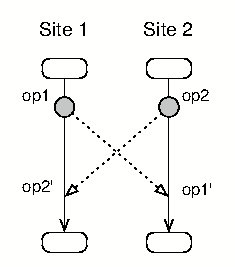
\includegraphics[scale=0.5]{OT-Operations-Order.jpg}
	\caption{order of operations for different sites}
\end{figure}

\end{frame}


\begin{frame}{Transformation Matrix}
\framesubtitle{formal definition}

\[o_{j}^{'} = T(o_j, o_i, p_j, p_i)\]
\[o_{i}^{'} = T(o_i, o_j, p_i, p_j)\]
\center{then \textbf{T} is such that following is satisfied:}

\[o_{j}^{'} \odot o_{i}^{'} = o_{i}^{'} \odot o_{j}^{'}\]


\end{frame}


\begin{frame}{Transformation Function picture}

\begin{figure}
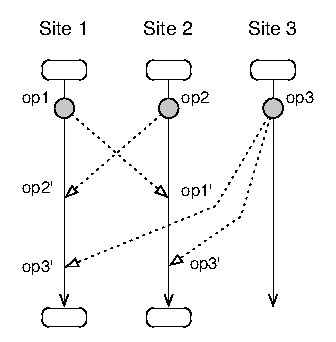
\includegraphics[scale=0.5]{OT-Transformation-Matrix.jpg}
\caption{Transformation Function}
\end{figure}

\end{frame}



\begin{frame}{OT Summary: Intention-violation}

\begin{itemize}
	\item Famous algos: GROVE, dOPT, Jupiter, adOPTed, REDUCE, GOT, GOTO
	\item Proving correctness of transformation functions is a complex task
	\item Impossible to establish proofs without computer within reasonable time for complex TF
	\item Following Oster et al. "Proving correctness of transformation functions in collaborative editing systems" paper only OT implementation of Tombstone Transformation Functions is correct
\end{itemize}
\end{frame}


\begin{frame}{Who is using OT?}

\begin{itemize}
	\item Google Docs
	\item ex-Google Wave
	\item A lot of other experiments
\end{itemize}
\end{frame}


\begin{frame}{OT Ressel et al. model}

\begin{columns}[c]
  \begin{column}{0.1\textwidth}    	
  \end{column}

  \begin{column}{0.4\textwidth}  
    \begin{figure}
      \centering    
	  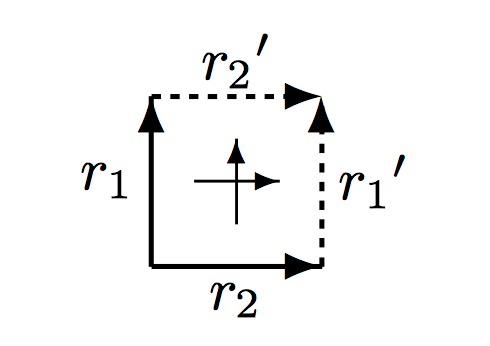
\includegraphics[scale=0.3]{OT-MatthiasRessel-2.png}    
      \caption{L-Transformation: $r_1 \odot r_2^{'} \equiv r_2 \odot r_1^{'}$}
    \end{figure}
  \end{column}

  \begin{column}{0.5\textwidth}
    \begin{center}
      \begin{figure}
        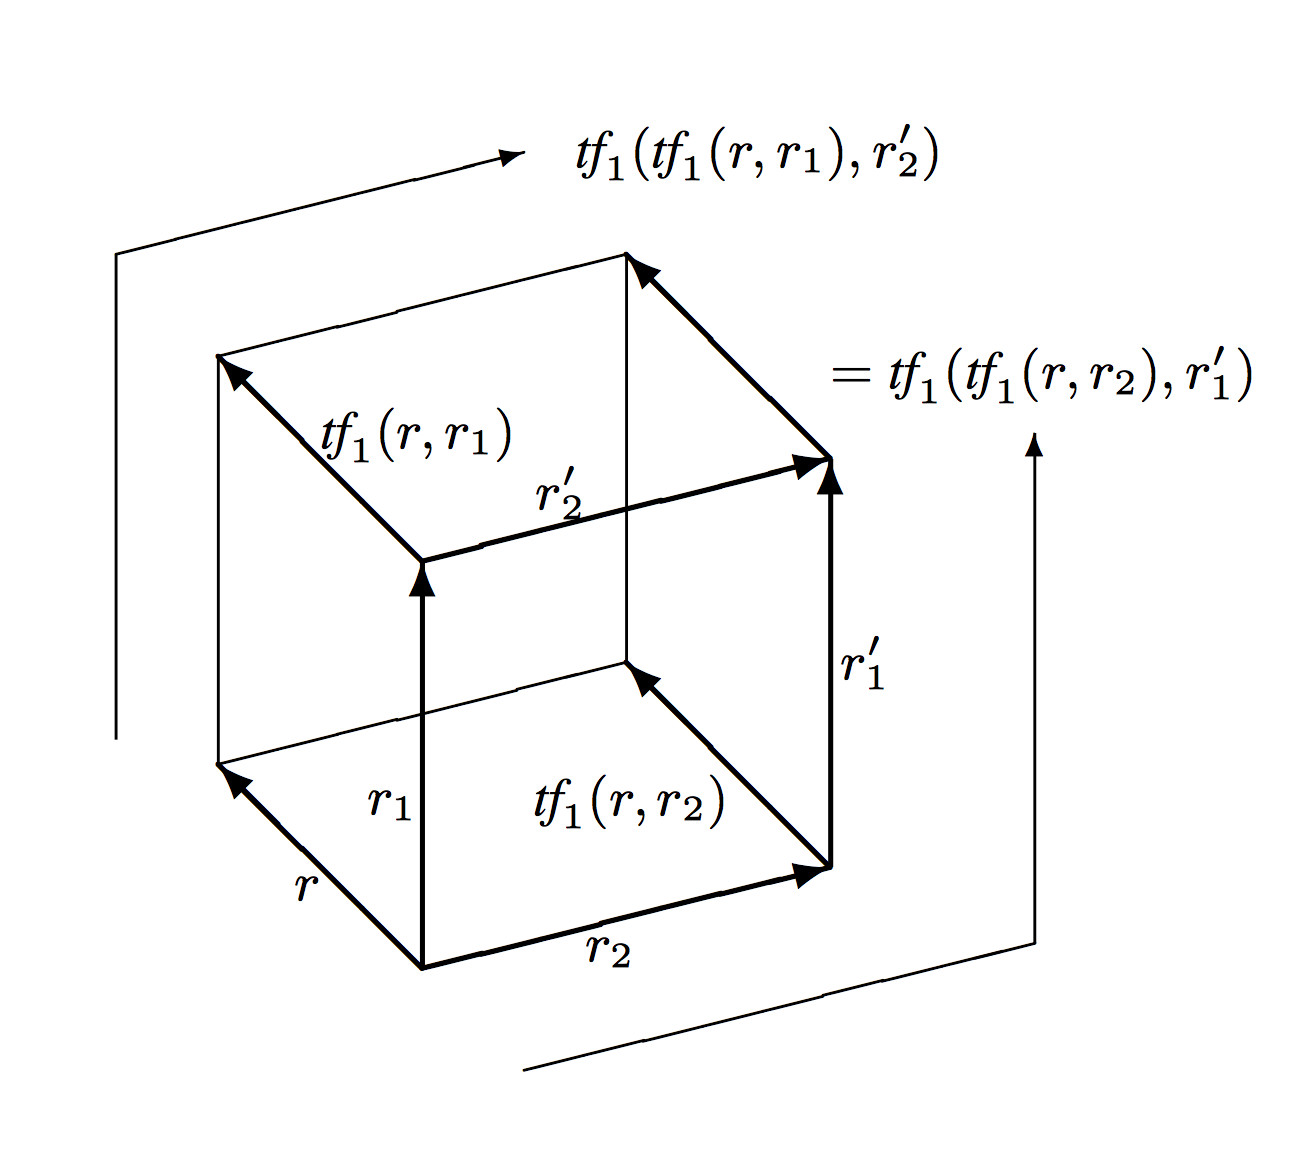
\includegraphics[scale=0.25]{OT-MatthiasRessel-1.png}
      \end{figure}
    \end{center}
  \end{column}
\end{columns}	

\end{frame}



\begin{frame}{Conflict-free replicated data types (CRDT)}
\begin{block}{CRDT is}
data type for the system of processes interconnected by an asynchronous network
where replicas can be updated independently and concurrently without coordination
between the replicas.
\end{block}
\vspace{0.5cm}
This kind of replication is very handy for client-side developers because:
\begin{itemize}
	\item Does not require active back-end system participation
	\item Quality leap in UX for users with weak or blinking network connections
	\item Better experience for SPAs with long single-load sessions like SoundCloud or GMail
	\item Offline work
\end{itemize}
\end{frame}


\begin{frame}{CRDTs: CvRDT, CmRDT}
\framesubtitle{state-based and op-based replication}

\begin{columns}[c]
  \begin{column}{0.4\textwidth}  
    \begin{figure}
      \centering    
	  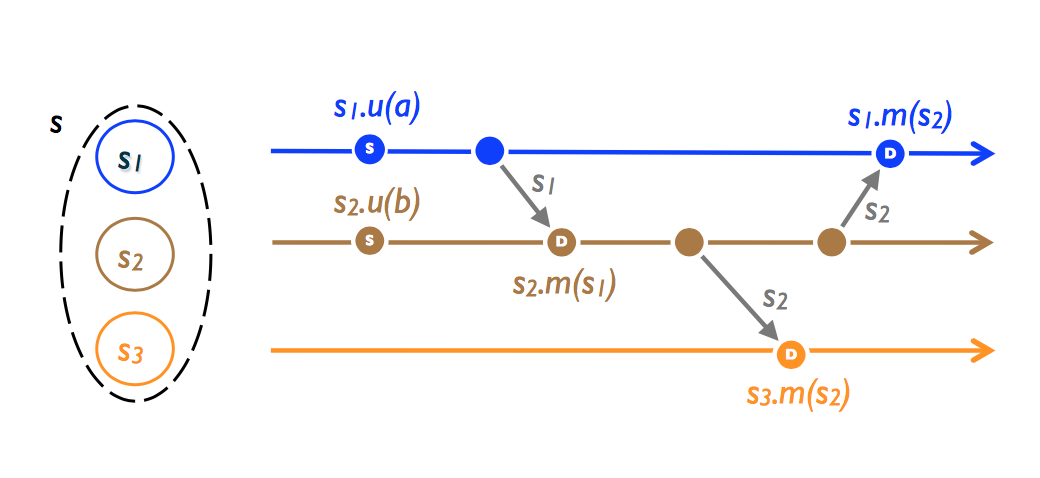
\includegraphics[scale=0.3]{CRDT-StateBased.png}    
      \caption{\textbf{State-based} Convergent Replicated Data Type or CvRDT}
    \end{figure}
  \end{column}

  \begin{column}{0.4\textwidth}
    \begin{center}
      \begin{figure}
        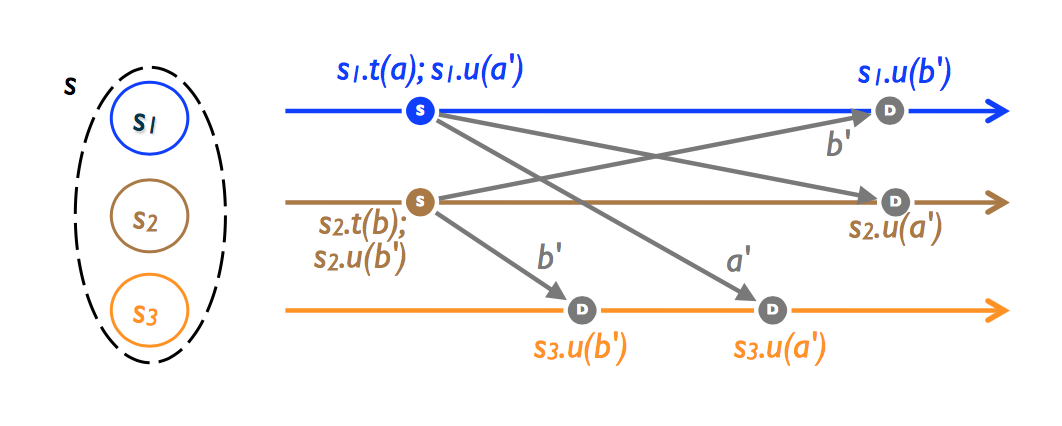
\includegraphics[scale=0.3]{CRDT-OP-Based.png}
        \caption{\textbf{Op-based} Commutative Replicated Data Type or CmRDT}
      \end{figure}
    \end{center}
  \end{column}
\end{columns}	


\end{frame}


\begin{frame}{CvRDT and CmRDT Properties}
\framesubtitle{Required properties}

In Abstract Algebra a CRDT is formally known as a Semilattice.
All Semilattices must have the following properties:

\begin{itemize}
	\item \textbf{commutativity} – $\forall x, y : x \odot y = y \odot x$
	\item \textbf{associativity} – nodes must come to the exactly same state regardless of the order they receive information: $x \odot (y \odot z) = (x \odot y) \odot z$
	\item \textbf{idempotency} – $x \odot x = x$
\end{itemize}

\begin{figure}[!ht]
	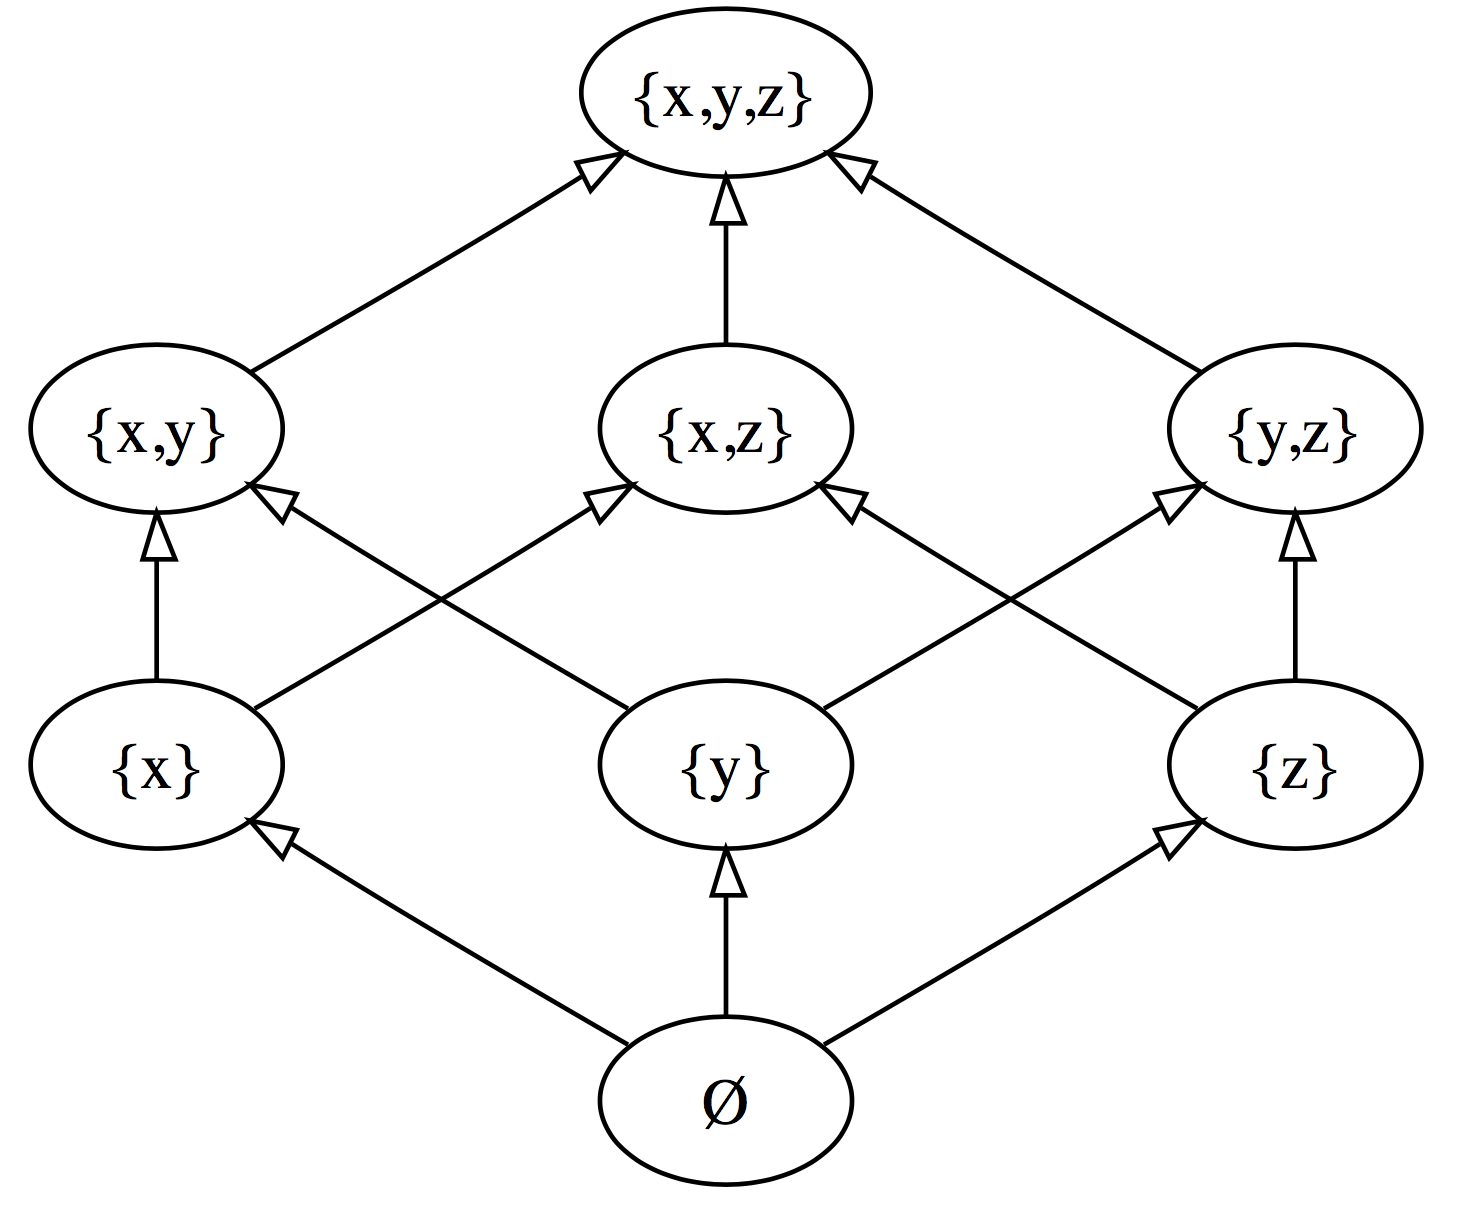
\includegraphics[scale=0.15]{LUB.png}    
	\caption{Least Upper Bound}
\end{figure}

\end{frame}


\begin{frame}{CRDT: Types}
\framesubtitle{Registers, Counters, Sets}

\begin{itemize}
  \item Register: LWW or Multi-Value (Dynamo or Couchdb-like)
  \item Counter (growth-only) and Counter w/decrementing
  \item G-Set – growth-only set
  \item 2P-Set – remove only once set (G-Set + Tombstones set)
  \item LWW-Element-Set – vector clocks 
  \item OR-Set – unique-tagged elements and list of tags within Tombstones set
  \item Treedoc, Logoot etc.
\end{itemize}
\end{frame}


\begin{frame}{CRDT: GCounter}
\framesubtitle{Increment only counter}

\inputminted[
  firstline=1,
  framesep=0.5cm,
  frame=leftline,
  baselinestretch=1.1,
  fontsize=\scriptsize,
  rulecolor=\color{white}  
  linenos=true]{javascript}{gcounter.js}

\end{frame}

\begin{frame}{CRDT: PNCounter}
\framesubtitle{Increment and decrement counter}

\inputminted[
  firstline=1,
  framesep=0.5cm,
  frame=leftline,
  baselinestretch=1.1,
  fontsize=\scriptsize,
  rulecolor=\color{white}
  linenos=true]{javascript}{pncounter.js}
  
\end{frame}


\begin{frame}{CRDT: PNCounter Test}
\framesubtitle{Increment and decrement counter}

\inputminted[
  firstline=1,
  framesep=0.01cm,
  frame=leftline,
  baselinestretch=1.1,
  fontsize=\scriptsize,
  rulecolor=\color{white}
  linenos=true]{javascript}{pncounter-test.js}
\end{frame}


\begin{frame}{CRDT: PNCounter example output}

\inputminted[
  firstline=1,
  framesep=0.5cm,
  frame=leftline,
  baselinestretch=1.1,
  fontsize=\scriptsize,
  rulecolor=\color{white}
  linenos=true]{text}{output-pncounter.js.txt}
  
\end{frame}

\begin{frame}{Existing Tools}

\begin{itemize}
  \item ShareDB (and fall of Google Wave)
  \item Swarm (and forever-in-pre-alpha tool)
  \item OT.js (Operational Transformation for JS)
  \item CRDT – github.com/dominictarr/crdt
  \item replikativ.io – p2p distributed system framework
  \item other CRDT implementations
\end{itemize}

\end{frame}


\begin{frame}{Who is using CRDTs?}
\begin{itemize}
	\item \href{https://dzone.com/articles/facebook-announces-apollo-qcon}{Facebook}
	\item \href{https://speakerdeck.com/ajantis/practical-demystification-of-crdts}{TomTom}
	\item \href{http://highscalability.com/blog/2014/10/13/how-league-of-legends-scaled-chat-to-70-million-players-it-t.html}{League of Legends}
	\item \href{https://developers.soundcloud.com/blog/roshi-a-crdt-system-for-timestamped-events}{SoundCloud}
	\item \href{http://www.erlang-factory.com/static/upload/media/1434558446558020erlanguserconference2015bet365michaelowen.pdf}{Bet265}
	\item \href{http://docs.basho.com/riak/kv/2.2.3/developing/data-types/}{RIAK Distributed Database}
\end{itemize}
\end{frame}


\begin{frame}{Drawbacks of CRDT}
\framesubtitle{you can't pour two buckets of shit into one bucket}
However, a major drawback in current state-based CRDTs is \textbf{the communication overhead of shipping the entire state}, which can get very large in size. For instance, the size of a counter CRDT (a vector of integer counters, one per replica) \textit{increases with the number of replicas}; whereas in a grow-only Set, the state size depends on the set size, that grows as more operations are invoked.
\end{frame}

\begin{frame}{$\delta$-mutation}
\framesubtitle{Everything at a cost}

\begin{itemize}
	\item “state fragments” merged using desired semantics
	\item ${\delta}$-mutators, defined in such a way to return a delta-state, typically, with a much smaller size than the full state.
\end{itemize}

\center
\textbf{\href{https://github.com/CBaquero/delta-enabled-crdts}{delta-enabled-crdts}} 
\end{frame}


\begin{frame}{References}

\begin{thebibliography}{9}
\setbeamertemplate{bibliography item}[text]
\bibitem{1}
Marc Shapiro, Nuno Pregui ̧ca, Carlos Baquero, Marek Zawirski. 
\textit{A comprehensive study of Convergent and Commutative Replicated Data Types.}
\setbeamertemplate{bibliography item}[text]
\bibitem{2}
Yasushi Saito, Marc Shapiro
\textit{Replication: Optimistic Approaches}

\setbeamertemplate{bibliography item}[text]
\bibitem{3}
Mihai Let, Nuno Pregui, Marc Shapiro
\textit{CRDTs: Consistency without concurrency control∗}

\setbeamertemplate{bibliography item}[text]
\bibitem{4}
Giuseppe DeCandia, Deniz Hastorun, Madan Jampani, Gunavardhan Kakulapati, Avinash Lakshman, Alex Pilchin, Swaminathan Sivasubramanian, Peter Vosshall and Werner Vogels
\textit{Dynamo: Amazon’s Highly Available Key-value Store}

\setbeamertemplate{bibliography item}[text]
\bibitem{5}
G ́erald Oster, Pascal Urso, Pascal Molli, Abdessamad Imine. 
\textit{Real time group editors without Operational transformation.}

\setbeamertemplate{bibliography item}[text]
\bibitem{6}
Gérald Oster, Pascal Urso†, Pascal Molli, Abdessamad Imine
\textit{Proving correctness of transformation functions in collaborative editing systems}

\end{thebibliography}	

\end{frame}




\begin{frame}
\begin{thebibliography}{99}

\setbeamertemplate{bibliography item}[text]
\bibitem{7}
Paulo S ́ergio Almeida, Ali Shoker, and Carlos Baquero
\textit{Efficient State-based CRDTs by Delta-Mutation}

\setbeamertemplate{bibliography item}[text]
\bibitem{8}
A. Bieniusa, M. Zawirski, N. Preguiça, M. Shapiro, Carlos Baquero, Valter Balegas, Sérgio Duarte.
\textit{An Optimized Conflict-free Replicated Set.}

\setbeamertemplate{bibliography item}[text]
\bibitem{9}
C.A. Ellis, S.J. Gibbs
\textit{Concurrency Control in Groupware Systems}

\setbeamertemplate{bibliography item}[text]
\bibitem{10}
Pascal Molli, Ge ́rald Oster
\textit{Using the Transformatinal Approach to Build a Safe and Generic Data Synchronizer}


\setbeamertemplate{bibliography item}[text]
\bibitem{11}
Pascal Molli, Ge ́rald Oster
\textit{Using the Transformatinal Approach to Build a Safe and Generic Data Synchronizer}

\setbeamertemplate{bibliography item}[text]
\bibitem{12}
Paulo S ́ergio Almeida, Ali Shoker, and Carlos Baquero
\textit{Delta State Replicated Data Types}, 2016


\end{thebibliography}	
\end{frame}



\begin{frame}
\center{Thanks}
\center{@maxmaxmaxmax}

\vspace{1cm}
\begin{footnotesize}
\href{https://github.com/joymax/odessajs2017}{https://github.com/joymax/odessajs2017}
\end{footnotesize}

\end{frame}

\end{document}


